\section{Auswertung}
\label{sec:Auswertung}

\subsection{Magnetfeld von Spulen}
\subsubsection{Kurze Spule}
\label{sec:1}
In diesem Abschnitt wird die gemessene Magnetfeldstärke auf der radialsymmetrischen 
Achse von der kleinen und einer großen Spule mit den theoretischen Werten für die 
erwartete Magnetfeldstärke verglichen.
\begin{table}[H]
    \centering
    \caption{Messwerte der kurzen Spule.}
    \label{tab:t1}
    %\sisetup{table-format=1.1, per-mode=reciprocal}
    \begin{tblr}{
        colspec = {S S},
        row{1} = {guard, mode=math},
      }
      \toprule
      \text{x} (\unit{\centi\meter}) & \text{Magnetfeldstärke} (\unit{\tesla}) \\
      \midrule
      0   &0.083\\
      1   &0.112\\
      2   &0.154\\
      3   &0.230\\
      4   &0.399\\
      5   &0.727\\
      6   &1.282\\
      7   &1.703\\
      8   &2.053\\
      9   &2.105\\
      10  &1.981\\
      11  &1.589\\
      12  &1.029\\
      13  &0.558\\
      14  &0.332\\
      15  &0.192\\
      16  &0.126\\
      \bottomrule
    \end{tblr}
\end{table}
\autoref{tab:t1} sind die aufgenommenen Messwerte der Magnetfeldstärke auf der Achse 
der kleinen Spule zu entnehmen. x ist der Abstand von einem Punkt aus, welcher 5 \unit{\centi\meter} von 
der Spule entfernt liegt, durch die Spule durch bis 5 \unit{\centi\meter} aus der Spule herraus. Des weiteren 
sind die Messwerte in \autoref{fig:1} graphisch dargestellt.
\begin{figure}
    \caption{Magnetische Feldstärke auf der Achse der kurzen Spule}
    \label{fig:1}
    \centering
    \includegraphics{"build/plot1.pdf"}
\end{figure}
Wenn man bedenkt, dass der eintrit der Hall sonde in das Magnetfeld fünf \unit{\centi\meter} 
von $x = 0$ entfernt liegt und auch nach dem Austritt $5$ weitere Messwerte aufgenommen wurden, 
kann man die restlichen Messwerte, die in der Spule aufgenommen, Mitteln um das Magnetfeld im 
innern der Spule zu berechnen. Damit kommt man zu einer Feldstärke von 
\begin{equation*}
    \symbf{B}_{exp} = \qty{1.63(0.18)}{\milli\tesla}.
\end{equation*}
Die Theoretische Magnetfeldstärke im inneren der Spule kann mit \autoref{eqn:4} Bestimmt werden.
Mit den Werten $ I = 1\unit{\ampere}$,$ n = 100 $ und einer Länge von ca 8\unit{\centi\meter}
ergibt sich 
\begin{equation*}
    \symbf{B}_{theo} = \qty{1.57e-3}{\tesla} = \qty{1.57}{\milli\tesla}
\end{equation*}

%%%%%%%%%%%%%%%%%%%%%%%%%%%%%%%%%%%%%%%%%%%%%%%%%%%%%%%%%%%%%%%%%%%%%%%%%%%%%%%%%%%%%%%%%%%%%%%%%
\subsubsection{Lange Spule}
Bei der Ermittlung der Magnetfeldstärke in der Langen Spule wird genauso verfahren, wie schon 
in \autoref{sec:1}.
\begin{table}[H]
    \centering
    \caption{Messwerte der langen Spule.}
    \label{tab:t2}
    %\sisetup{table-format=1.1, per-mode=reciprocal}
    \begin{tblr}{
        colspec = {S S},
        row{1} = {guard, mode=math},
      }
      \toprule
      x (\unit{\centi\meter}) & Magnetfeldstärke (\unit{\tesla}) \\
      \midrule
      0   &0.019\\
      1   &0.041\\
      2   &0.072\\
      3   &0.136\\
      4   &0.253\\
      5   &0.503\\
      6   &0.971\\
      7   &1.544\\
      8   &1.978\\
      9   &2.192\\
      10  &2.279\\
      11  &2.333\\
      12  &2.360\\
      13  &2.379\\
      14  &2.382\\
      15  &2.379\\
      16  &2.368\\
      17  &2.340\\
      18  &2.301\\
      19  &2.231\\
      20  &2.286\\
      21  &2.184\\
      22  &1.965\\
      23  &1.552\\
      24  &0.977\\
      25  &0.519\\
      26  &0.297\\
      27  &0.190\\
      28  &0.133\\
      29  &0.101\\
      30  &0.081\\
      \bottomrule
    \end{tblr}
\end{table}

\begin{figure}
    \caption{Magnetische Feldstärke auf der Achse der langen Spule}
    \label{fig:1}
    \centering
    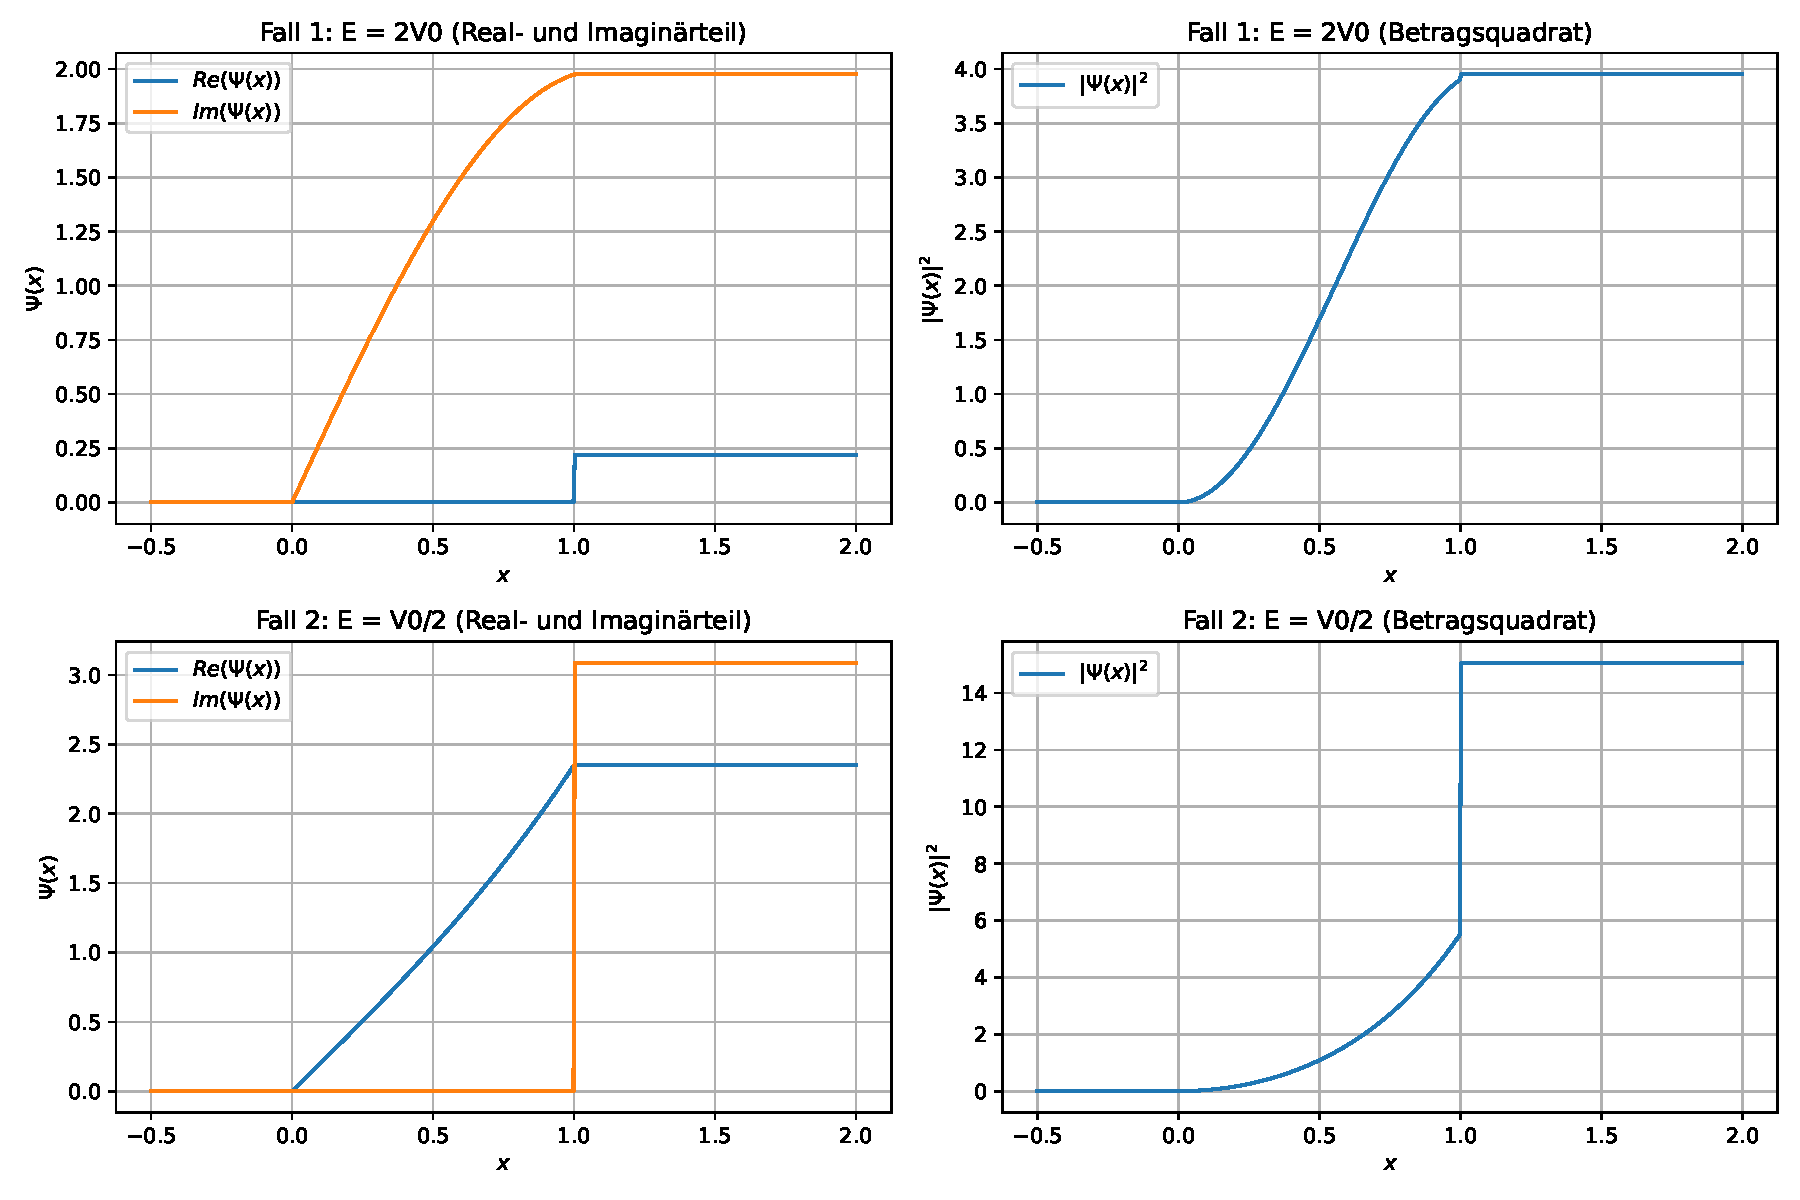
\includegraphics{"build/plot2.pdf"}
\end{figure}
Aus den Messwerten kann analog zu der kleinen  Spule das Magnetfeld innerhalb der Spule 
gemitelt werden, um so einen experimentellen wert für die Magnetfeldstärke im inneren 
der Spule zu erhalten.So erhällt man
\begin{equation*}
    \symbf{B}_{exp,lang} = \qty{1.90(0.13)}{\milli\tesla}.
\end{equation*}
Der Theoretische Wert der Spule mit Länge $l = 19\unit{\centi\meter} $ wird nach 
\autoref{eqn:4} bestimmt.
\begin{equation*}
    \symbf{B}_{exp,lang} = \qty{1.98e-3}{\tesla} = \qty{1.98}{\milli\tesla}.
\end{equation*}

%%%%%%%%%%%%%%%%%%%%%%%%%%%%%%%%%%%%%%%%%%%%%%%%%%%%%%%%%%%%%%%%%%%%%%%%%%%%%%%%%%%%%%%%%%%%%%%%%%%%%
\begin{table}[H]
    \centering
    \caption{Messwerte Hysteresekurve.}
    \label{tab:t3}
    %\sisetup{table-format=1.1, per-mode=reciprocal}
    \begin{tblr}{
        colspec = {S S },
        row{1} = {guard, mode=math},
      }
      \toprule
      I (\unit{\ampere}) & B(\unit{\milli\tesla}) \\
      \midrule
      0 &  1\\
    1  & 90\\
    2  & 260\\
    3  & 390\\
    4  & 479\\
    5  & 540\\
    4  & 516\\
    3  & 483\\
    2  & 430\\
    1  & 308\\
    0  & 122\\
    -1 & -80\\
    -2 & -258\\
    -3 & -395\\
    -4 & -482\\
    -5 & -540\\
    -4 & -515\\
    -3 & -483\\
    -2 & -429\\
    -1 & -305\\
    0  & -117\\
    1  & 79\\
    2  & 259\\
    3  & 392\\
    4  & 479\\
    5  & 340 \\
    \bottomrule
    \end{tblr}
\end{table}
\subsection{Hysteresekurve}
Über die aufgenommenen Messwerte der Magnetfeldstärke im Luftspalt der ringspule soll hier 
die Sättigungsmagnetisierung, Remanenz und Koerzitivkraft bestimmt werden.
\begin{figure}[H]
    \caption{Hysteresekurve}
    \label{fig:3}
    \centering
    \includegraphics{"build/plot3.pdf"}
\end{figure}
Die Werte der Remananz kann man der Tabellle \autoref{}





%%%%%%%%%%%%%%%%%%%%%%%%%%%%%%%%%%%%%%%%%%%%%%%%%%%%%%%%%%%%%%%%%%%%%%%%%%%%%%%%%%%%%%%%%%%%%%%
Den Tabellen \autoref{} und \autoref{} sind die Werte für die Magnetfeldstärke auf der 
Symetrieachse eines Helmholzspulenpaares einmal für große und einmal für kleine 
Abstände der Spulen zu entnehmen. $x$ in $\unit{\milli\meter} $ ist dabei der Abstand 
vom linken ende der skala der Hall Sonde. Um die Darstellung und den Vergleich mit der 
Theoriekurve zu vereinfachen wurde die $x$-Skala so verschoben, dass der Nullpunkt jewails 
in der Mitte der beiden Spulen liegt.
\subsection{Helmholzspulenpaar}
\begin{figure}
    \caption{Magnetfeldstärke Spulenpaar $19\unit{\centi\meter}$ Abstand}
    \label{fig:4}
    \centering
    \includegraphics{"build/plot4.pdf"}
\end{figure}

\begin{figure}
    \caption{Magnetfeldstärke Spulenpaar $8\unit{\centi\meter}$ Abstand}
    \label{fig:5}
    \centering
    \includegraphics{"build/plot5.pdf"}
\end{figure}